\section{Inference in First-Order Logic}
	On va voire comment les algo font pour répondre une question FOL
	\subsection{Propositional vs FOL inference}
		\textbf{Universal Instantiation (UI)} Pour n'importe quelle phrase $\alpha$ , variables $v$, et \textit{ground term} $g$ (terme sans variables)
		
		\begin{equation}
			\cfrac{\forall v \ \alpha}{subst(\{v/g\}, \alpha)}
		\end{equation}
		
		$v$ peut etre remplacer par n'importe quelle instance

		$subst(\omega,\alpha)$ applique la substitution $\omega$ sur $\alpha$
		
		ex : 
		
		$\forall x King(x) \land Greedy(x) \Rightarrow Evil(x)$ Avec on peut déduire que $King(Bob) \land Greedy(Bob) \Rightarrow Evil(Bob)$
		
		\textbf{Existential instantiation}
		Pour n'importe quelle phrase $\alpha$ , variables $v$, et nouveau symbole constant $k$
			\begin{equation}
				\cfrac{\exists \ \alpha}{subst(\{v/k\}, \alpha)}
			\end{equation}
		
		$v$ peut etre remplacé avec un nouveau symbole
		
		ex :
		
		$\exists x  \ mother(bob,x)$ on peut déduire $mother(Bob, ANewMother)$
		
		$ANewMother$ est un constante de Skolem, équivalence déductive (pas d'équivalence logique)
		
		Avec ces deux instantiations, on peut réduire FOL a des symboles de propositions.
		
		\subsubsection{Reduction to Propositional Logic}	
			Le problème est que il y a une infinité de \textit{ground terms} mais grace a Herbrand, on sait que :
			
			\textit{If a sentence $\alpha$ is entailed by a FOL KB, it's entailed by a \textbf{finite} subset of the propositionalized KB}
			
			Application $n=0$ a $\infty$:
			\begin{itemize}
				\item creer un KB propositionnelle en l'instanciant avec un terme de profondeur $n$
				\item regarder si $\alpha$ est entaillé par le KB
			\end{itemize}
			
			Si $\alpha$ est pas entaillé l'algo loop a l'infini
			
			\textbf{Turing} : Entaillement pour FOL est semidécidable
			
	\subsection{Unification}
		C'est une substitution qui fait que des expression logique différente semble identique
		
		ex : 
		
		Parent(Bob,x) et Parent(y,z)
		\begin{itemize}
			\item \{y/Bob, x/z\} : Parent(Bob,z)
			\item \{y/Bob, x/Lucia, z/Lucia\} : Parent(Bob, Lucia)
		\end{itemize}	
		
		L'algo $Unify(p,q)$ prend 2 phrase atomique $p$ et $q$ et retourne une sibstitution qui fait que $p$ et $q$ sont identique.
		
		$Unify(p,q) = \emptyset$ où $Subst(\emptyset, p) = Subst(\emptyset, q)$
		
		$\emptyset$ est l' unificateur des 2 phrases. il y en possiblement plus que 1
		
		\subsubsection{Most General Unifier}
			MGU pour les KOG, fait que "la substitution qui s'engage le moins sur les les variables contraignantes"
			
			ex : 
			
			$Unify(Parent(Bob,x),Parent(y,z)) = \{y/Bob, x/z\}$
			
			MGU est unique
			
		
		\subsubsection{Standardize apart}
			Si 2 phrase partages des variables alors on peut les unifiers, pour eviter les conflits de noms, on renome un des variables.
			
			$Unify(Paren(Bob,x), Parent(y,z)) = Unify(Parent(Bob,w), Parent(q,r))$
		
			\begin{figure}[htp]	
				\centering
				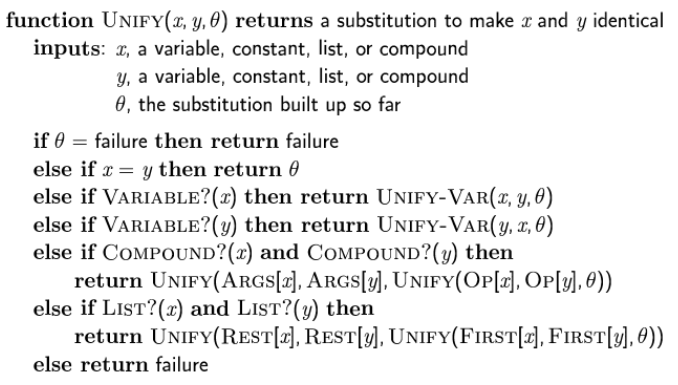
\includegraphics[width=0.7\textwidth]{img/Unification.png}
				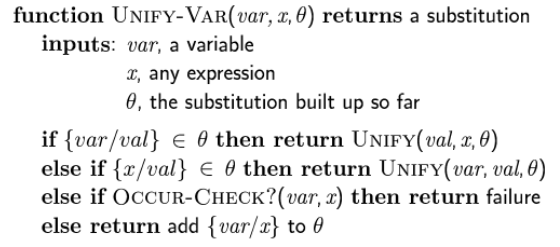
\includegraphics[width=0.7\textwidth]{img/Unification1.png}
			\end{figure}
			
		\subsubsection{Generalized Modus Ponens}
			avec $Subst(\emptyset, p_i) = Subst(\emptyset,p_i')$ pour tous les I
			\begin{equation}
				\cfrac{p_1', p_2',\dots,p_n',(p_1 \land,p_2 \land \dots \land p_n \Rightarrow q)}{Subst(\emptyset, q)}
			\end{equation}
			
			ex :
			
			\begin{equation}
			\cfrac{King(Bob), Greedy(y), (King(x) \land Greedy(y) \Rightarrow Evil(x))}{Evil(Bob)}
			\end{equation}
			Avec $\emptyset = \{x/Bob, y/Bob\}$	
			
	\subsection{Forward Chaining}z
		\subsubsection{First-order definite clauses}

		\begin{itemize}
			\item Trouver toutes les regles dont les prémisses sont satisfaites
			\item Ajouter leurs conclusions au faits connus
			\item Repréter l'opération jusqu'a ce qu'une réponse soit apportée a la question  ou qu'aucun fait nouveau n'est ajouté
			
		\end{itemize}	
		
		\begin{figure}[htp]	
			\centering
			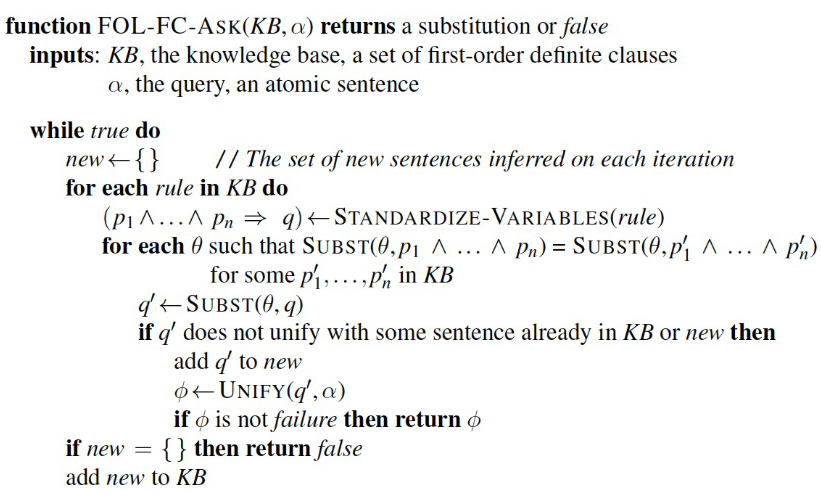
\includegraphics[width=0.7\textwidth]{img/ForwardChaining.png}
		\end{figure}		
		
		\subsubsection{Analyse}
			\textbf{Soundness :} Il ne dérive que les phrases qui sont impliquées, parce que Generalize Modus Ponen le fait.
			
			\textbf{Completeness :} Il répond à toutes les requêtes dont les réponses sont impliquées par le KB, mais peut ne pas se terminer en raison de la semi-décidabilité de l'implication avec des clauses définies.
			
	\subsection{Backward chaining}
		Commence  avec les prémisses de l'objectif
		\begin{itemize}
			\item Chaque prémisses doit etre supporté par le KB
			\item Commencer avec la premieres hypotheses et chercher soutient du KB
			
		\end{itemize}
		
		La fonctions est un algo récursive tel que une depth-first.
		
		\begin{figure}[htp]	
			\centering
			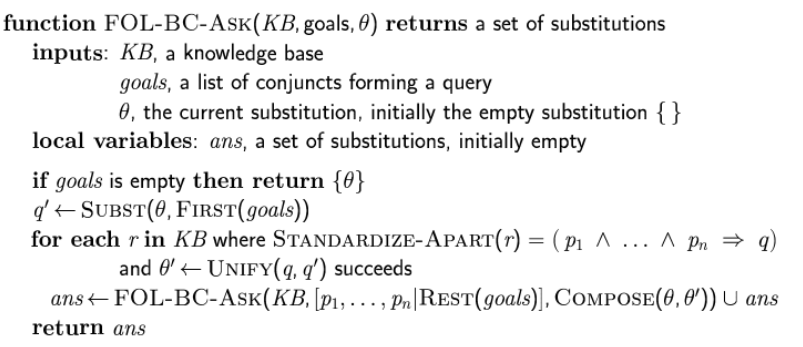
\includegraphics[width=0.7\textwidth]{img/BackWardChaining.png}
		\end{figure}		
		
		\subsubsection{Logic programming: Prolog}
			Algorithm = Logic + Control
			
			TODO
			
	\subsection{Résolutions}
		Chaque phrase d'un FOL peut etre convertit en CNF (conjuctive Normal Form)
			
		\begin{enumerate}
			\item \textbf{Eliminer Implications} : $p \Rightarrow q$ devient $\neg  \lor q$ 
			\item \textbf{Bouger  les $\neg$ qui sont devant}  :
			\begin{itemize}
				\item $\neg(p\lor q)$ devient $\neg p \land \neg q$
				\item $\neg(p\land q)$ devient $\neg p \lor \neg q$
				\item $\neg \forall x, p$ devient $ \exists x \ \neg p$
				\item $\neg \exists x, p$ devient $\forall x\  \neg p$
				\item $\neg \neg p$ devient $p$
			\end{itemize}
			\item \textbf{standardiser les variables} : $(\forall x P(x)) \lor (\exists x \ Q(x))$ devient $(\forall x P(x)) \lor (\exists y \ Q(y))$
			\item \textbf{Bouger les quantifiers a gauche} : $p \lor \forall x \ q$ devient $\forall x \ p \lor q$
			\item \textbf{Skolemization} : Voire prochaine sections
			\item \textbf{De Morgan}
		\end{enumerate}
		
		\subsubsection{Skilemization}
			Objectif est de:
			\begin{itemize}
				\item retirer tous les quantifiers existants
				\item Replacer les varaibles par des toutes nouvelles constantes qui n'existe pas de le KB
			\end{itemize}			 
			
			ex : $\exists x \ Q(x)$ devient $Q(A)$ avec où $A$ est unique
			
			Pour les phrases plus complexe, on utilise des fonctions de symbole (Skolem functions) pour indiquer des valeur  spécifique.
			
			ex : $\forall Animal(x,A)$ devient $\forall Animal(x,F(x))$
			
		\subsubsection{Resolution inference rule}
			Pour $p_i$ and $q_i$ où $UNIFY(p_j, \neg q_k) = \emptyset$
			\begin{equation}
				\cfrac{p_1 \lor \dots p_j \dots \lor p_m, q_1 \lor \dots p_k \dots \lor q_n}{SUBST(\emptyset,(p_1 \lor \dots p_{j-1} \lor p_{j+1} \dots \lor p_m \lor q_1 \lor \dots q_{k-1} \lor q_{k+1} \dots \lor q_n))}
			\end{equation}
			
			exemple plus concret :
			
			\begin{figure}[htp]	
				\centering
				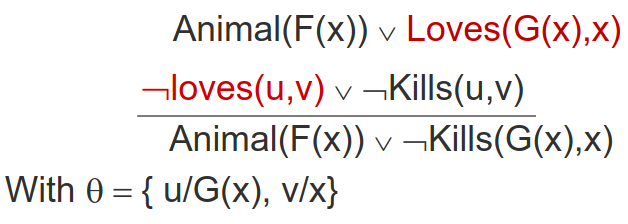
\includegraphics[width=0.5\textwidth]{img/RIR.png}
			\end{figure}	
			
			$\alpha$ est un conséquence logique de KB si KB $\models \alpha$ IFF ($KB \land \neg \alpha$) insatisfait
			
			On transforme juste $\neg \alpha$ en CNF et montre que $KB \land \alpha$ insatisfait car apres application des règles de résolutions.
			
			\begin{figure}[htp]	
				\centering
				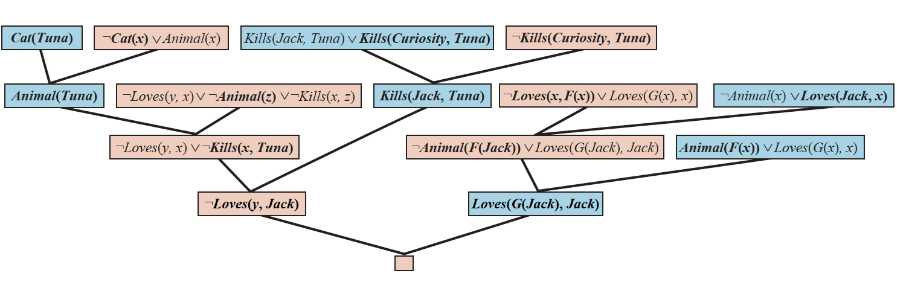
\includegraphics[width=0.9\textwidth]{img/RIR1.png}
			\end{figure}
			
		\subsubsection{Introducing answers}
		
			\begin{figure}[htp]	
				\centering
				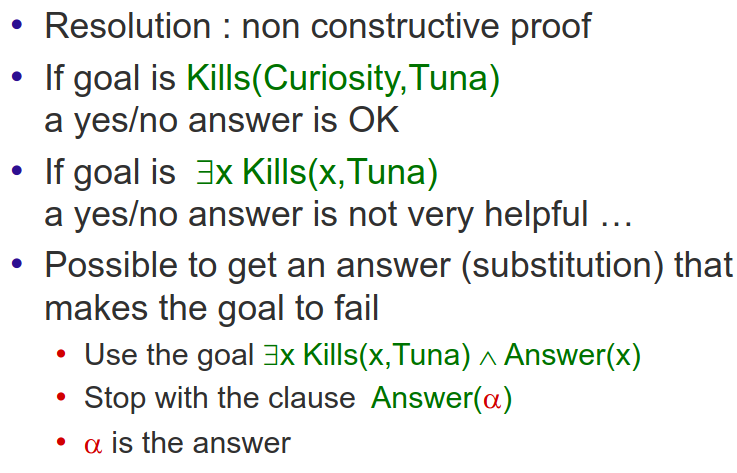
\includegraphics[width=0.8\textwidth]{img/RIR2.png}
			\end{figure}\section{Inference in First-Order Logic}
	On va voire comment les algo font pour répondre une question FOL
	\subsection{Propositional vs FOL inference}
		\textbf{Universal Instantiation (UI)} Pour n'importe quelle phrase $\alpha$ , variables $v$, et \textit{ground term} $g$ (terme sans variables)
		
		\begin{equation}
			\cfrac{\forall v \ \alpha}{subst(\{v/g\}, \alpha)}
		\end{equation}
		
		$v$ peut etre remplacer par n'importe quelle instance

		$subst(\omega,\alpha)$ applique la substitution $\omega$ sur $\alpha$
		
		ex : 
		
		$\forall x King(x) \land Greedy(x) \Rightarrow Evil(x)$ Avec on peut déduire que $King(Bob) \land Greedy(Bob) \Rightarrow Evil(Bob)$
		
		\textbf{Existential instantiation}
		Pour n'importe quelle phrase $\alpha$ , variables $v$, et nouveau symbole constant $k$
			\begin{equation}
				\cfrac{\exists \ \alpha}{subst(\{v/k\}, \alpha)}
			\end{equation}
		
		$v$ peut etre remplacé avec un nouveau symbole
		
		ex :
		
		$\exists x  \ mother(bob,x)$ on peut déduire $mother(Bob, ANewMother)$
		
		$ANewMother$ est un constante de Skolem, équivalence déductive (pas d'équivalence logique)
		
		Avec ces deux instantiations, on peut réduire FOL a des symboles de propositions.
		
		\subsubsection{Reduction to Propositional Logic}	
			Le problème est que il y a une infinité de \textit{ground terms} mais grace a Herbrand, on sait que :
			
			\textit{If a sentence $\alpha$ is entailed by a FOL KB, it's entailed by a \textbf{finite} subset of the propositionalized KB}
			
			Application $n=0$ a $\infty$:
			\begin{itemize}
				\item creer un KB propositionnelle en l'instanciant avec un terme de profondeur $n$
				\item regarder si $\alpha$ est entaillé par le KB
			\end{itemize}
			
			Si $\alpha$ est pas entaillé l'algo loop a l'infini
			
			\textbf{Turing} : Entaillement pour FOL est semidécidable
			
	\subsection{Unification}
		C'est une substitution qui fait que des expression logique différente semble identique
		
		ex : 
		
		Parent(Bob,x) et Parent(y,z)
		\begin{itemize}
			\item \{y/Bob, x/z\} : Parent(Bob,z)
			\item \{y/Bob, x/Lucia, z/Lucia\} : Parent(Bob, Lucia)
		\end{itemize}	
		
		L'algo $Unify(p,q)$ prend 2 phrase atomique $p$ et $q$ et retourne une sibstitution qui fait que $p$ et $q$ sont identique.
		
		$Unify(p,q) = \emptyset$ où $Subst(\emptyset, p) = Subst(\emptyset, q)$
		
		$\emptyset$ est l' unificateur des 2 phrases. il y en possiblement plus que 1
		
		\subsubsection{Most General Unifier}
			MGU pour les KOG, fait que "la substitution qui s'engage le moins sur les les variables contraignantes"
			
			ex : 
			
			$Unify(Parent(Bob,x),Parent(y,z)) = \{y/Bob, x/z\}$
			
			MGU est unique
			
		
		\subsubsection{Standardize apart}
			Si 2 phrase partages des variables alors on peut les unifiers, pour eviter les conflits de noms, on renome un des variables.
			
			$Unify(Paren(Bob,x), Parent(y,z)) = Unify(Parent(Bob,w), Parent(q,r))$
		
			\begin{figure}[htp]	
				\centering
				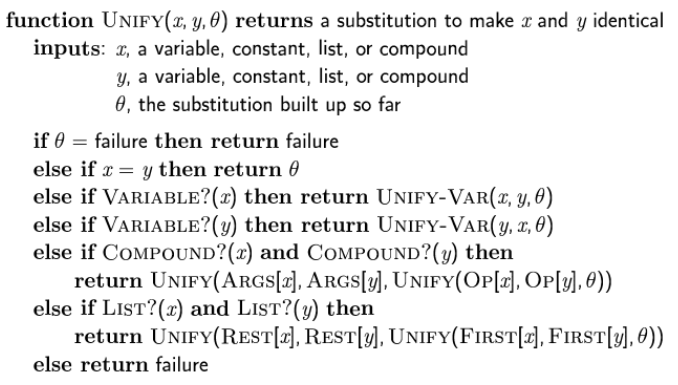
\includegraphics[width=0.7\textwidth]{img/Unification.png}
				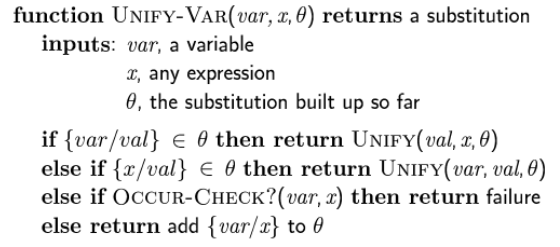
\includegraphics[width=0.7\textwidth]{img/Unification1.png}
			\end{figure}
			
		\subsubsection{Generalized Modus Ponens}
			avec $Subst(\emptyset, p_i) = Subst(\emptyset,p_i')$ pour tous les I
			\begin{equation}
				\cfrac{p_1', p_2',\dots,p_n',(p_1 \land,p_2 \land \dots \land p_n \Rightarrow q)}{Subst(\emptyset, q)}
			\end{equation}
			
			ex :
			
			\begin{equation}
			\cfrac{King(Bob), Greedy(y), (King(x) \land Greedy(y) \Rightarrow Evil(x))}{Evil(Bob)}
			\end{equation}
			Avec $\emptyset = \{x/Bob, y/Bob\}$	
			
	\subsection{Forward Chaining}z
		\subsubsection{First-order definite clauses}

		\begin{itemize}
			\item Trouver toutes les regles dont les prémisses sont satisfaites
			\item Ajouter leurs conclusions au faits connus
			\item Repréter l'opération jusqu'a ce qu'une réponse soit apportée a la question  ou qu'aucun fait nouveau n'est ajouté
			
		\end{itemize}	
		
		\begin{figure}[htp]	
			\centering
			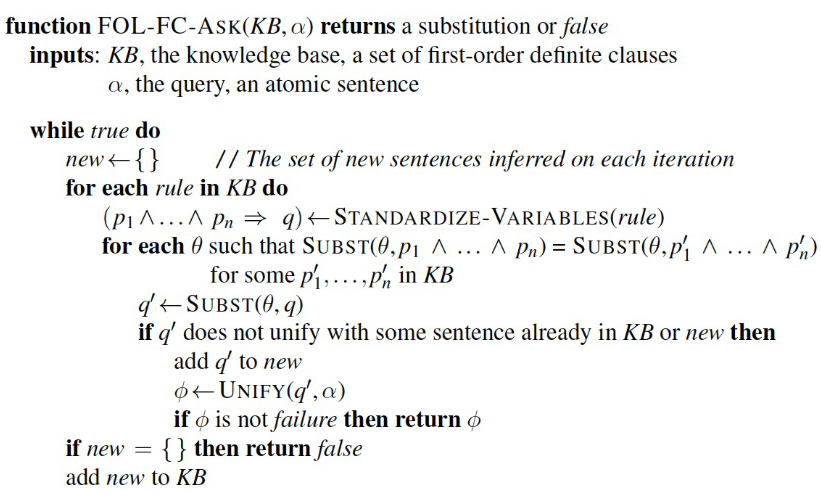
\includegraphics[width=0.7\textwidth]{img/ForwardChaining.png}
		\end{figure}		
		
		\subsubsection{Analyse}
			\textbf{Soundness :} Il ne dérive que les phrases qui sont impliquées, parce que Generalize Modus Ponen le fait.
			
			\textbf{Completeness :} Il répond à toutes les requêtes dont les réponses sont impliquées par le KB, mais peut ne pas se terminer en raison de la semi-décidabilité de l'implication avec des clauses définies.
			
	\subsection{Backward chaining}
		Commence  avec les prémisses de l'objectif
		\begin{itemize}
			\item Chaque prémisses doit etre supporté par le KB
			\item Commencer avec la premieres hypotheses et chercher soutient du KB
			
		\end{itemize}
		
		La fonctions est un algo récursive tel que une depth-first.
		
		\begin{figure}[htp]	
			\centering
			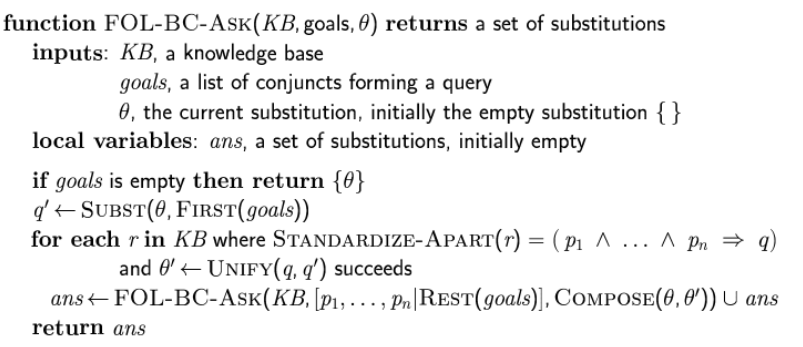
\includegraphics[width=0.7\textwidth]{img/BackWardChaining.png}
		\end{figure}		
		
		\subsubsection{Logic programming: Prolog}
			Algorithm = Logic + Control
			
			TODO
			
	\subsection{Résolutions}
		Chaque phrase d'un FOL peut etre convertit en CNF (conjuctive Normal Form)
			
		\begin{enumerate}
			\item \textbf{Eliminer Implications} : $p \Rightarrow q$ devient $\neg  \lor q$ 
			\item \textbf{Bouger  les $\neg$ qui sont devant}  :
			\begin{itemize}
				\item $\neg(p\lor q)$ devient $\neg p \land \neg q$
				\item $\neg(p\land q)$ devient $\neg p \lor \neg q$
				\item $\neg \forall x, p$ devient $ \exists x \ \neg p$
				\item $\neg \exists x, p$ devient $\forall x\  \neg p$
				\item $\neg \neg p$ devient $p$
			\end{itemize}
			\item \textbf{standardiser les variables} : $(\forall x P(x)) \lor (\exists x \ Q(x))$ devient $(\forall x P(x)) \lor (\exists y \ Q(y))$
			\item \textbf{Bouger les quantifiers a gauche} : $p \lor \forall x \ q$ devient $\forall x \ p \lor q$
			\item \textbf{Skolemization} : Voire prochaine sections
			\item \textbf{De Morgan}
		\end{enumerate}
		
		\subsubsection{Skilemization}
			Objectif est de:
			\begin{itemize}
				\item retirer tous les quantifiers existants
				\item Replacer les varaibles par des toutes nouvelles constantes qui n'existe pas de le KB
			\end{itemize}			 
			
			ex : $\exists x \ Q(x)$ devient $Q(A)$ avec où $A$ est unique
			
			Pour les phrases plus complexe, on utilise des fonctions de symbole (Skolem functions) pour indiquer des valeur  spécifique.
			
			ex : $\forall Animal(x,A)$ devient $\forall Animal(x,F(x))$
			
		\subsubsection{Resolution inference rule}
			Pour $p_i$ and $q_i$ où $UNIFY(p_j, \neg q_k) = \emptyset$
			\begin{equation}
				\cfrac{p_1 \lor \dots p_j \dots \lor p_m, q_1 \lor \dots p_k \dots \lor q_n}{SUBST(\emptyset,(p_1 \lor \dots p_{j-1} \lor p_{j+1} \dots \lor p_m \lor q_1 \lor \dots q_{k-1} \lor q_{k+1} \dots \lor q_n))}
			\end{equation}
			
			exemple plus concret :
			
			\begin{figure}[htp]	
				\centering
				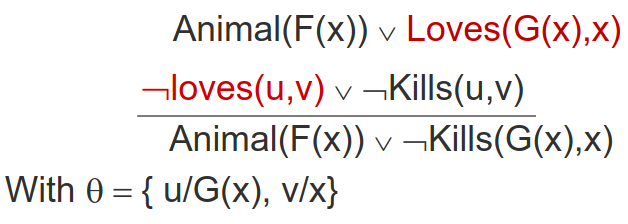
\includegraphics[width=0.5\textwidth]{img/RIR.png}
			\end{figure}	
			
			$\alpha$ est un conséquence logique de KB si KB $\models \alpha$ IFF ($KB \land \neg \alpha$) insatisfait
			
			On transforme juste $\neg \alpha$ en CNF et montre que $KB \land \alpha$ insatisfait car apres application des règles de résolutions.
			
			\begin{figure}[htp]	
				\centering
				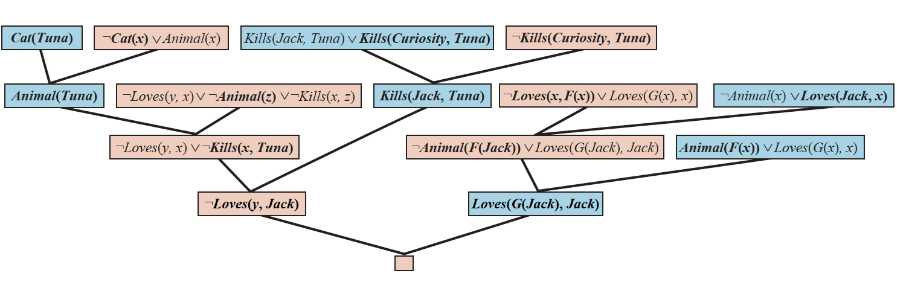
\includegraphics[width=0.9\textwidth]{img/RIR1.png}
			\end{figure}
			
		\subsubsection{Introducing answers}
		
			\begin{figure}[htp]	
				\centering
				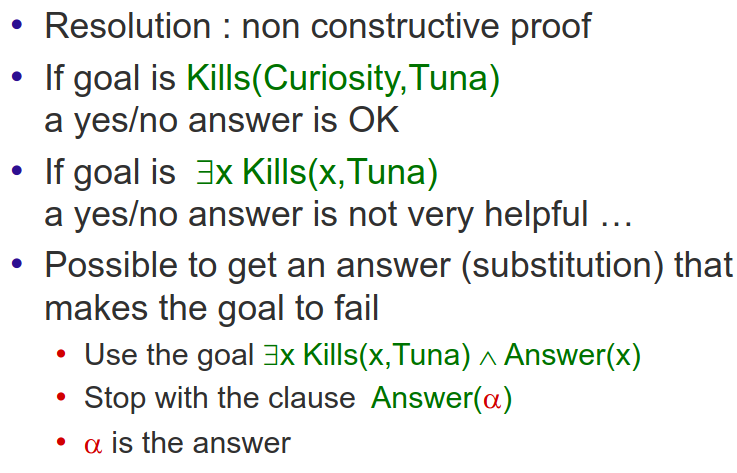
\includegraphics[width=0.8\textwidth]{img/RIR2.png}
			\end{figure}